\documentclass[11pt]{article}
\usepackage[margin=1in]{geometry}
\usepackage{amsmath,amssymb}
\usepackage{graphicx}
\usepackage{booktabs,tabularx,multirow}
\usepackage[table]{xcolor}
\usepackage{siunitx}
\usepackage{enumitem}
\usepackage{caption}
\usepackage{float}
\usepackage[most]{tcolorbox}
\usepackage{tikz}
\usepackage{circuitikz}
\usetikzlibrary{arrows.meta,positioning,calc,fit}
\usepackage{listings}
\usepackage{microtype}
\usepackage{fancyhdr}
\usepackage[colorlinks=true,linkcolor=blue!45!black,citecolor=blue!45!black,urlcolor=blue!45!black]{hyperref}

\sisetup{detect-all}
\setlist{itemsep=2pt,topsep=3pt}
\captionsetup{font=small,labelfont=bf}
\definecolor{accent}{RGB}{190,30,45}

\newtcolorbox{keybox}[1]{colback=white,colframe=black!75,boxrule=0.6pt,arc=1pt,
  title=#1,fonttitle=\bfseries,coltitle=white,colbacktitle=black!75,left=6pt,right=6pt,top=4pt,bottom=4pt}
\newtcolorbox{checkbox}[1]{colback=yellow!6,colframe=orange!70!black,boxrule=0.5pt,arc=1pt,
  title=#1,fonttitle=\bfseries\small,coltitle=black,colbacktitle=orange!25,left=6pt,right=6pt,top=3pt,bottom=3pt}

\lstset{basicstyle=\ttfamily\scriptsize,columns=fullflexible,breaklines=true,frame=single,rulecolor=\color{black!40},
  xleftmargin=4pt,xrightmargin=4pt,language=Verilog,keywordstyle=\bfseries,commentstyle=\itshape\color{black!60}}

\pagestyle{fancy}\fancyhf{}
\lhead{\small Keeper-side allocation for lower metastability $\tau$}
\rhead{\small Handoff document v0.1 --- 26 Sep 2026}
\cfoot{\small\thepage}

\newcommand{\tauF}{\tau}
\newcommand{\gf}{g_{\mathrm{f}}}
\newcommand{\gk}{g_{\mathrm{k}}}
\newcommand{\Cq}{C_{\mathrm{mq}}}
\newcommand{\Cqb}{C_{\mathrm{mqb}}}

\begin{document}

\begin{center}
{\LARGE\bfseries Where the Strength Goes:\\[3pt] Reducing Flip-Flop Metastability by Keeper-Side Allocation}\\[8pt]
{\large Design, theory, GF180 simulation evidence and test-chip plan}\\[4pt]
{\large Project handoff document (ECE 298A, Tiny Tapeout GF180MCU)}\\[10pt]
Benjamin J.\ Eisenberg \quad Roshan [surname]\\[2pt]
University of Waterloo \quad 26 September 2026 \quad Revision 0.1 (for iteration)
\end{center}

\begin{keybox}{The claim in one paragraph}
A flip-flop resolves metastability (decides between 0 and 1 after its input changed too close to the clock edge)
at a rate set by its master latch: the time constant $\tau$ of the latch's unstable mode, the time for a small
imbalance to grow by a factor $e\approx2.72$. In the latch, $\tau$ depends on the \emph{geometric mean} of its two stages' drive-to-capacitance ratios, so the weak
stage dominates. (The \emph{forward} stage passes the stored value on; the \emph{keeper} feeds it back to hold it.)
Our allocation law follows: \textbf{adding drive to the weak (keeper) stage shortens $\tau$;
adding drive to the already-strong (forward) stage lengthens it, even though it adds transistors.} In GF180MCU
SPICE at five process--voltage conditions, strengthening the keeper cuts $\tau$ by 10.9--12.6\% (4.8\% at the
slow corner), strengthening the forward stage raises $\tau$ by 11.5--14.0\%, and a flip-flop built from standard
NAND cells with the favourable allocation has 36--47\% lower $\tau$ than the library \texttt{dffq\_1} (the NAND topology alone gives 33--39\%). Because
$\tau$ sits in the exponent of the mean time between failures (MTBF: the average time between moments when a
synchronizer is still undecided when it is read), with 2\,ns of settling time (TT, 3.3\,V, equal prefactors) these become a
$45\times$ MTBF gain over our baseline and $4.5\times10^{6}$ over the library flip-flop. The test chip measures
all four flip-flops on one die with the on-chip early/late method of Beer et al.\ \cite{beer2011}.
\end{keybox}

\noindent\textbf{How to read this document.} New to metastability? Read the primer in Section~\ref{sec:background}
and the story of how we arrived at the idea in Section~\ref{sec:story} first; they define every term used later.
Sections~\ref{sec:law}--\ref{sec:evidence} give the theory and the evidence; Section~\ref{sec:instrument} the chip.

\tableofcontents
\newpage

%=====================================================================
\section{Executive summary}
\begin{itemize}
\item \textbf{Problem.} Wherever a signal passes between parts of a chip that run on unrelated clocks (a clock-domain
  crossing), flip-flops called \emph{synchronizers} catch it. They sometimes catch it mid-change and need extra time
  to decide. The chance they are still undecided after waiting a settling time $S$ falls as $e^{-S/\tau}$, so $\tau$
  sets reliability exponentially. Measured $\tau$ in modern
  processes is worse than scaling predicts: about 100\,ps in 65\,nm against an expected $<30$\,ps \cite{beer2010}.
\item \textbf{Known remedies and their limit.} Published guidance \cite{beer2015} improves $\tau$ from the outside
  (supply, threshold voltage, removing reset and scan, loading, duty cycle). Adding feedback \emph{inside} the
  flip-flop has made $\tau$ worse in silicon: Beer et al.\ found the standard library flip-flop had lower $\tau$
  than several feedback-enhanced flip-flops \cite{beer2011}.
\item \textbf{Our contribution.} (i) An allocation law that says where added drive helps and where it hurts, with a
  first-order criterion (Section~\ref{sec:law}). (ii) A realization with standard cells only: a NAND master--slave
  flip-flop whose loop strengths we choose. (iii) GF180 SPICE evidence at five conditions
  (Section~\ref{sec:evidence}). (iv) A test chip that measures the baseline, the keeper-strengthened, the
  forward-strengthened and the library flip-flop side by side (Section~\ref{sec:instrument}).
\item \textbf{Evidence (SPICE).} Ordering $\tau_{\text{keeper}\uparrow} < \tau_{\text{baseline}} <
  \tau_{\text{forward}\uparrow}$ holds at all five conditions. The full $3\times3$ sweep of forward and keeper
  strengths obeys ``strengthen the weaker stage'' in all six one-dimensional sweeps (Figure~\ref{fig:law}).
\item \textbf{Status.} Circuits and instrument frozen; the delay line is sized from measured GF180 delays (two estimated, see Section~\ref{sec:instrument}).
  Next: RTL integration, proposal talk (1 Oct), design review (8 Oct), shuttle close (7 Dec 2026).
\item \textbf{Main risk.} Silicon may differ from SPICE; the chip is built to measure the predicted differences
  (5--13\% keeper against baseline, 12--14\% forward against baseline, 19--29\% forward against keeper) with a target
  ratio precision of $\pm3\%$.
\end{itemize}

%=====================================================================
\section{Background: metastability and why $\tau$ matters}
\label{sec:background}
\begin{keybox}{Primer: the terms used in this document}
\begin{description}[leftmargin=0pt,itemsep=2pt,font=\normalfont\bfseries]
\item[Flip-flop.] A one-bit memory that copies its input D to its output Q at the rising clock edge. Inside are two
  latches, the \emph{master} and the \emph{slave}. Each latch is a loop of two inverting gates that holds a value by
  feeding it back to itself.
\item[Metastability.] If D changes almost exactly at the clock edge, the master latch is left partway between 0 and 1,
  like a ball balanced on a hilltop. It must roll off to one side; the closer to the top it starts, the longer it takes.
\item[Balance point.] The data timing that leaves the latch exactly on the hilltop. We call its offset from the clock
  edge $\delta^*$, and the distance of an actual data edge from it $u$.
\item[$\tau$ (tau).] The time for the latch's small imbalance to grow by a factor $e\approx2.72$ while it rolls off.
  Smaller $\tau$ means faster decisions.
\item[Synchronizer.] A flip-flop that receives a signal from another clock domain. Its input timing is random, so
  metastability cannot be avoided there, only given time to resolve.
\item[Settling time $S$.] How long the design waits before the next flip-flop reads the synchronizer, typically
  about one clock period (nanoseconds).
\item[Failure and MTBF.] A failure is the synchronizer still being undecided when it is read; the next circuit may
  then see garbage. The mean time between failures (MTBF) is the average time between such events. Designs aim for
  years to millennia.
\item[Drive and load.] A gate's drive is its transconductance $g$: how much current its output pushes per volt of
  input change. A node's load is its capacitance $C$: how much charge it must receive to change its voltage. The
  latch's $\tau$ is roughly $C/g$: a heavy load slows it and strong drive speeds it up.
\item[Forward and keeper.] The two gates in a latch loop. The forward gate passes the value on (here to the slave);
  the keeper feeds it back so the latch holds it.
\item[Corners.] The foundry's typical (TT), slow (SS) and fast (FF) transistor models. Simulating at each, and at
  3.0, 3.3 and 3.6\,V, checks that a result survives normal chip-to-chip and supply variation.
\end{description}
\end{keybox}

When a flip-flop's data input changes too close to its clock edge, its master latch is left near its balance point
with a small differential voltage $x_0 = V_1 - V_2$. The latch then regenerates. Linearized about the balance point,
\begin{equation}
C\,\frac{dx}{dt} = g\,x \quad\Longrightarrow\quad x(t) = x_0\,e^{t/\tau},\qquad \tau = \frac{C}{g},
\label{eq:lin}
\end{equation}
with $g$ the net regenerative transconductance and $C$ the node capacitance. The time to reach a valid logic level
$x_{\mathrm{valid}}$ is $t_{\mathrm{res}} = \tau\ln(x_{\mathrm{valid}}/|x_0|)$, which grows without bound as $x_0\to0$.
For a synchronizer that allows settling time $S$, with clock frequency $f_C$, data transition rate $f_D$ and
metastability window $T_W$,
\begin{equation}
\mathrm{MTBF}(S) = \frac{e^{S/\tau}}{f_C\,f_D\,T_W}.
\label{eq:mtbf}
\end{equation}
Two flip-flops with time constants $\tau'$ and $\tau$ and the same prefactor therefore differ by
\begin{equation}
\frac{\mathrm{MTBF}'}{\mathrm{MTBF}} = \exp\!\Big[S\Big(\frac{1}{\tau'}-\frac{1}{\tau}\Big)\Big].
\label{eq:ratio}
\end{equation}
A 10\% smaller $\tau$ at $S=20\tau$ multiplies MTBF by about $e^{2.2}\approx 9$; at $S=40\tau$ by about $85$.

\paragraph{Worked example.} With $S=2$\,ns, our baseline flip-flop ($\tau=64.5$\,ps) has $S/\tau=31.0$, and the
keeper-strengthened one ($\tau=57.5$\,ps) has $S/\tau=34.8$. The exponents differ by 3.8, so by \eqref{eq:ratio} the
MTBF differs by $e^{3.8}\approx45$. An 11\% change in $\tau$ becomes a $45\times$ change in reliability because
every $\tau$ of waiting divides the failure chance by $e$, and the faster flip-flop fits 3.8 more $\tau$ into the
same 2\,ns.
This exponential leverage is why $\tau$ is the parameter worth improving \cite{ginosar2011}.

\paragraph{What cannot help.} The failure probability is
$P(\text{unresolved at } S) \approx T_W f_D\, e^{-\Lambda(S)}$ with $\Lambda(S)=\int_0^S dt/\tau(t)$. Only a larger
regeneration exponent $\Lambda$ (more drive per unit capacitance during resolution) or a smaller window $T_W$
(a constant factor only) helps. Input-independent noise, dither or ``kicks'' leave the density of initial
imbalances near zero unchanged and cannot help. The two resolution directions ($0\!\to\!1$, $1\!\to\!0$) share one
unstable eigenvalue in the linear regime, so they share one $\tau$.

%=====================================================================
\section{How we arrived at the idea}
\label{sec:story}
This section explains the reasoning in the order it happened, including the ideas we dropped, so a reader can check
each step.

\begin{figure}[H]
\centering
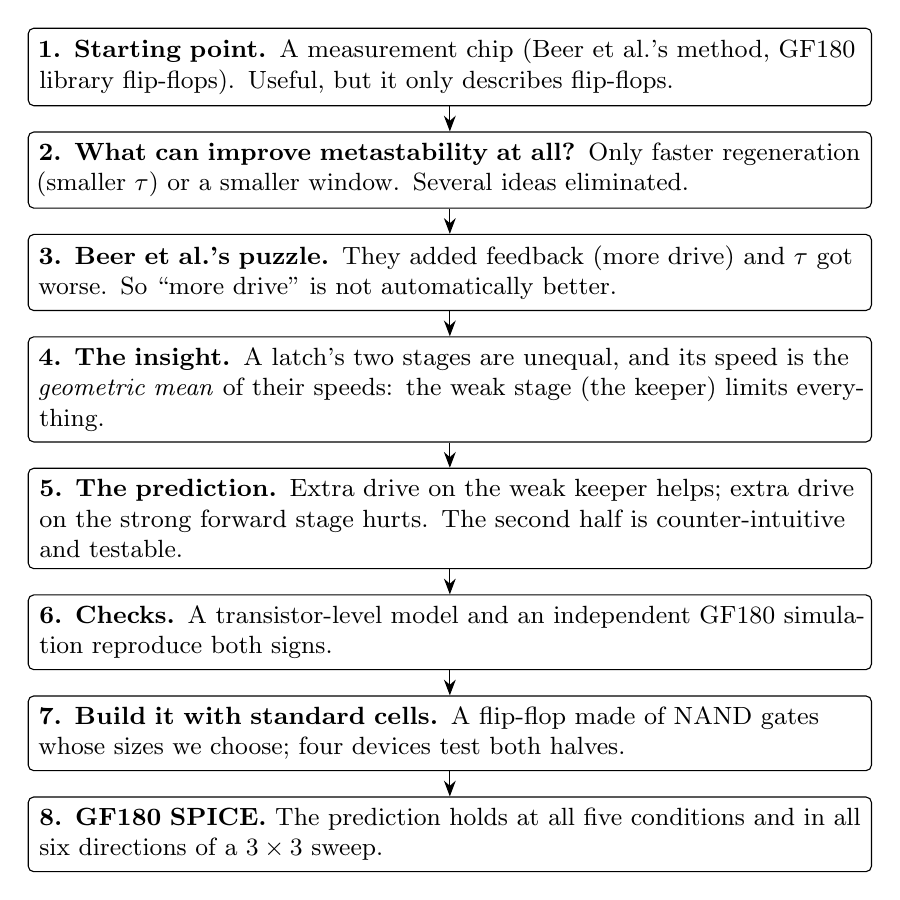
\begin{tikzpicture}[font=\small, node distance=3.2mm,
  st/.style={draw, rounded corners=2pt, align=left, text width=0.86\linewidth, inner sep=4pt},
  arr/.style={-{Stealth[length=2mm]}}]
\node[st] (a) {\textbf{1. Starting point.} A measurement chip (Beer et al.'s method, GF180 library flip-flops). Useful, but it only describes flip-flops.};
\node[st, below=of a] (b) {\textbf{2. What can improve metastability at all?} Only faster regeneration (smaller $\tau$) or a smaller window. Several ideas eliminated.};
\node[st, below=of b] (c) {\textbf{3. Beer et al.'s puzzle.} They added feedback (more drive) and $\tau$ got worse. So ``more drive'' is not automatically better.};
\node[st, below=of c] (d) {\textbf{4. The insight.} A latch's two stages are unequal, and its speed is the \emph{geometric mean} of their speeds: the weak stage (the keeper) limits everything.};
\node[st, below=of d] (e) {\textbf{5. The prediction.} Extra drive on the weak keeper helps; extra drive on the strong forward stage hurts. The second half is counter-intuitive and testable.};
\node[st, below=of e] (f) {\textbf{6. Checks.} A transistor-level model and an independent GF180 simulation reproduce both signs.};
\node[st, below=of f] (g) {\textbf{7. Build it with standard cells.} A flip-flop made of NAND gates whose sizes we choose; four devices test both halves.};
\node[st, below=of g] (h) {\textbf{8. GF180 SPICE.} The prediction holds at all five conditions and in all six directions of a $3\times3$ sweep.};
\foreach \x/\y in {a/b,b/c,c/d,d/e,e/f,f/g,g/h} \draw[arr] (\x) -- (\y);
\end{tikzpicture}
\caption{The path from a measurement chip to an improvement claim.}
\label{fig:story}
\end{figure}

\paragraph{Step 1: starting point.} The first plan was a measurement chip: build the on-chip early/late circuit of
Beer et al.\ \cite{beer2011} in GF180 and measure $\tau$ of two library flip-flops. That would give GF180 numbers,
but it would only describe flip-flops. We raised the bar: find a small change that makes $\tau$ smaller, with a
physical reason to expect it to work, and use the chip to test it.

\paragraph{Step 2: what can improve metastability at all?} The chance of failure is
$P\approx T_W f_D\,e^{-\Lambda(S)}$, with $\Lambda(S)=\int_0^S dt/\tau(t)$ (Section~\ref{sec:background}). Only two
things lower it: faster regeneration during the settling time (a larger exponent $\Lambda$, i.e.\ a smaller $\tau$),
or a narrower window $T_W$, which helps only by a constant factor. This eliminated several candidate ideas:
\begin{itemize}
\item \emph{Adding noise or a ``kick''} to push the latch off the hilltop: it pushes some latches that would have
  resolved back toward the top as often as it helps others; on average nothing changes.
\item \emph{Treating the 0$\to$1 and 1$\to$0 decisions separately}: both are the same unstable motion of the latch,
  with one $\tau$.
\item \emph{Storing the undecided value and resolving it later, or combining two samples}: this cannot beat the limit
  above; at best it acts as a preamplifier, which narrows $T_W$ by a constant.
\item \emph{Putting all extra load on one latch node}: correct in the idealized model, but only about 1--2\% in a
  transistor-level model.
\item \emph{Disconnecting the slave while the master resolves}: sound in theory, but it needs a custom transistor
  layout, which our standard-cell design cannot use.
\end{itemize}

\paragraph{Step 3: Beer et al.'s puzzle.} Beer et al.\ built flip-flops with extra feedback, which is extra drive, and
measured them: the plain library flip-flop had \emph{lower} $\tau$ than the feedback flip-flops \cite{beer2011}. The simple formula
$\tau=C/g$ says more drive ($g$) should help, but the added circuitry also added load ($C$). So the useful question is
not ``how much drive?'' but ``where does added drive help, and where does it hurt?''

\paragraph{Step 4: the insight.} A latch has two stages, and in an ordinary flip-flop they are deliberately unequal: the
forward gate is made strong so the flip-flop is fast, while the keeper, which only has to hold the value, is made small.
Writing the growth equations for two unequal stages (Section~\ref{sec:law}) gives
\[
\frac{1}{\tau}=\sqrt{\frac{\gf}{\Cq}\cdot\frac{\gk}{\Cqb}},
\]
the \emph{geometric mean} of the two stages' speeds (drive divided by load). A geometric mean is dominated by its
smaller factor: speeds 4 and 1 give 2, much closer to 1 than their average of 2.5. A weak keeper therefore limits the
whole latch, the way the weakest link limits a chain.

\paragraph{Step 5: the prediction.} Adding a transistor of a given width to a stage adds drive to that stage, but also
load on both latch nodes. Because of the geometric mean, what matters is the \emph{relative} change. Toy numbers make it
concrete: with forward drive 4 and keeper drive 1, adding one unit of drive doubles the keeper ($1\to2$) but raises the
forward stage by only 25\% ($4\to5$). Both additions bring roughly the same extra load. The keeper addition wins easily;
the forward addition gains so little that its extra load can outweigh it, and its gate load lands on the node that had
the least load, where it costs the most. Prediction: \textbf{strengthening the keeper shortens $\tau$; strengthening the
forward stage, the intuitive ``make it faster'' move, lengthens it.} This is consistent with Beer et al.'s result, though
proving it for their circuits needs their schematics.

\paragraph{Step 6: checks before building.} A transistor-level model (generic parameters) reproduced both signs: a
keeper assist cut $\tau$ by 23--36\%, the same width on the forward side raised it by 4--19\%. An independent GF180
simulation of a different latch, run separately, agreed in sign (84\,$\to$\,69\,ps and 95\,ps).

\paragraph{Step 7: making it buildable with standard cells.} A library flip-flop's internal sizes are fixed. We therefore
built our own flip-flop from NAND gates, whose sizes ($\times1$, $\times2$, $\times4$) we choose; two of them form the
master latch's forward and keeper stages. A first attempt with the library's tristate inverter was dropped because that
cell contains internal stages, which would put extra gates inside the loop. Four devices test the claim from both sides:
the library flip-flop, a baseline with a weak keeper, the same with a stronger keeper, and the same with a stronger
forward stage.

\paragraph{Step 8: GF180 simulation.} The prediction held at every condition tested, and the full $3\times3$ sweep of
forward and keeper sizes shows the rule in all six directions (Section~\ref{sec:evidence}). The chip now tests it in
silicon.

%=====================================================================
\section{The Beer et al.\ work and how this project relates}
\label{sec:beer}
\subsection{What Beer et al.\ did}
\begin{itemize}
\item \textbf{The devolution of synchronizers} \cite{beer2010}: measured $\tau\approx100$\,ps on a 65\,nm circuit,
  against $<30$\,ps expected from gate-delay scaling.
\item \textbf{On-chip measurement circuit} \cite{beer2011} (65\,nm, 1.1\,V): an all-digital circuit that clocks the
  flip-flop under test, samples its output once after a selectable short delay (early) and again much later
  (late), and counts early/late disagreements. The disagreement probability versus the early delay falls as
  $e^{-d/\tau}$; its slope gives $\tau$. They measured several synchronizers and reported that \emph{the standard
  library flip-flop had lower $\tau$ than various feedback flip-flops}, with SPICE agreeing that the regular
  flip-flop resolves faster than a transmission-gate feedback flip-flop.
\item \textbf{Eleven ways to boost your synchronizer} \cite{beer2015}: design guidance that treats the flip-flop
  cell as given: avoid scan and reset, use minimum-size cells, minimize routing and jitter, choose a
  high-performance process flavour and low threshold voltage, raise the supply, and adjust the clock duty cycle
  (the master and slave share the settling time, $\tau_{\mathrm{eff}}^{-1} = \alpha/\tau_M + (1-\alpha)/\tau_S$).
\end{itemize}

\subsection{How this project relates}
\begin{enumerate}
\item \textbf{We use their measurement method}, with credit: our chip is an early/late disagreement counter
  (Section~\ref{sec:instrument}).
\item \textbf{We answer the question their feedback result raises.} Extra feedback is extra drive, yet it made
  $\tau$ worse. Our law (Section~\ref{sec:law}) says added drive helps only if its relative gain in
  transconductance exceeds the relative capacitance it adds to the two latch nodes, and that this is easy on the
  weak stage and hard on the strong one. It predicts the opposite outcomes of the two placements, which our DUT3
  and DUT4 test directly.
\item \textbf{We act inside the flip-flop with standard cells.} Instead of accepting a library cell's internal
  sizing, we build the flip-flop from NAND gates whose strengths we choose, so the allocation is a design
  variable without custom layout.
\end{enumerate}

\begin{checkbox}{To confirm before the paper}
The specific $\tau$ values of Beer et al.'s feedback flip-flops (reported in our earlier notes as about 101\,ps
for the library flip-flop and 148--210\,ps for the feedback variants) and their schematics. The qualitative
result quoted above is taken from the paper's abstract. Whether our law explains \emph{their} variants needs their
schematics.
\end{checkbox}

%=====================================================================
\section{The allocation law}
\label{sec:law}
\subsection{Two-stage latch model}
\begin{figure}[t]
\centering
\begin{circuitikz}
\node[nand port] (F) at (0,1.2) {};
\node[nand port, xscale=-1] (K) at (0,-1.2) {};
\node[above=4pt] at (F.north) {\small forward NAND ($\gf$)};
\node[below=4pt] at (K.south) {\small keeper NAND ($\gk$)};
\coordinate (mq) at ($(F.out)+(2.0,0)$);
\coordinate (mqb) at ($(K.out)+(-3.0,0)$);
\draw (F.out) -- (mq);
\draw (K.out) -- (mqb);
\draw (mq) |- (K.in 1);
\draw (mqb) |- (F.in 1);
\fill (mq) circle (1.6pt) node[above=1pt] {\texttt{mq}};
\fill (mqb) circle (1.6pt) node[below=1pt] {\texttt{mqb}};
\draw (F.in 2) -- ++(-0.4,0) node[left] {\small $g_1{=}1$};
\draw (K.in 2) -- ++(0.4,0) node[right] {\small $g_2{=}1$};
\draw (mq) -- ++(2.6,0) node[right] {\small to slave};
\fill ($(mq)+(1.1,0)$) circle (1.3pt);
\draw ($(mq)+(1.1,0)$) to[C, l=$\Cq$] ++(0,-1.6) node[ground]{};
\draw (mqb) -- ++(-1.1,0) coordinate (cb);
\draw (cb) to[C, l_=$\Cqb$] ++(0,-1.6) node[ground]{};
\end{circuitikz}
\caption{Master latch of the NAND flip-flop during resolution (hold phase: both gating outputs are 1, so each loop
NAND acts as an inverter). The forward NAND drives \texttt{mq}, which also loads the slave; the keeper NAND drives
\texttt{mqb}. Loop feedback enters each NAND on pin A1.}
\label{fig:latch}
\end{figure}

Label the forward transconductance $\gf$ (drives \texttt{mq} from \texttt{mqb}) and the keeper transconductance $\gk$
(drives \texttt{mqb} from \texttt{mq}), with node capacitances $\Cq$ and $\Cqb$ (Figure~\ref{fig:latch}). Neglecting
output conductance and coupling capacitance,
\begin{equation}
\Cq\,\dot v_{\mathrm{mq}} = -\gf\, v_{\mathrm{mqb}},\qquad \Cqb\,\dot v_{\mathrm{mqb}} = -\gk\, v_{\mathrm{mq}}
\quad\Longrightarrow\quad
\frac{1}{\tau} = \lambda = \sqrt{\frac{\gf\,\gk}{\Cq\,\Cqb}} .
\label{eq:gm}
\end{equation}
In words: each node's voltage changes at a rate set by the drive of the gate feeding it divided by the node's load,
and the two nodes push each other in turn. The growth rate is therefore the geometric mean of the two stage rates
$\gf/\Cq$ and $\gk/\Cqb$. A weak stage limits $\tau$ in the way the weakest link limits a chain.

\subsection{First-order criterion}
Add width $w$ to the keeper. It adds transconductance $\Delta\gk = k w$, drain capacitance $c_d w$ on \texttt{mqb}
(the node it drives) and gate capacitance $c_g w$ on \texttt{mq} (the node it senses). From \eqref{eq:gm},
$\tau$ falls if and only if
\begin{equation}
\frac{\Delta\gk}{\gk} > \frac{\Delta\Cqb}{\Cqb} + \frac{\Delta\Cq}{\Cq}
\quad\Longleftrightarrow\quad
\frac{k}{\gk} > \frac{c_d}{\Cqb} + \frac{c_g}{\Cq}\quad\text{(to first order)}.
\label{eq:crit}
\end{equation}
The same criterion for the forward stage reads $k/\gf > c_d/\Cq + c_g/\Cqb$. In a flip-flop whose keeper is weak
($\gk \ll \gf$) the left side is large for the keeper and small for the forward stage. The forward stage also
places its gate capacitance on the lightly loaded node \texttt{mqb}, where the relative increase is largest.

\subsection{Exact linear model}
Number the nodes 1 = \texttt{mq} and 2 = \texttt{mqb}, so $C_1=\Cq$, $C_2=\Cqb$, $g_2=\gf$ (drives node 1) and
$g_1=\gk$ (drives node 2). With output conductances $G_1,G_2$ at the nodes and a coupling (Miller) capacitance $C_M$
between them, the unstable eigenvalue $\lambda$ is the positive root of
\begin{equation}
\lambda^2\big[C_1C_2 + C_M(C_1+C_2)\big] + \lambda\big[(C_1{+}C_M)G_2 + (C_2{+}C_M)G_1 + C_M(g_1{+}g_2)\big]
- (g_1g_2 - G_1G_2) = 0 .
\end{equation}
A transistor-level model with generic long-channel parameters (not GF180), Miller coupling and channel-length
modulation keeps the sign of the effect: a keeper-side assist of 0.5--2\,$\mu$m cut $\tau$ by 23--36\% while the same
width on the forward side raised it by 4--19\%. An independent GF180 simulation of a different master latch (a
clocked-inverter keeper), run separately during this project and not reproduced here, showed the same signs:
84\,$\to$\,69\,ps with a stronger keeper and 95\,ps with a stronger forward inverter.

\subsection{Statement of the law}
\begin{keybox}{Allocation law}
\begin{enumerate}[leftmargin=14pt]
\item Added drive on a latch stage shortens $\tau$ if and only if its relative gain in transconductance exceeds
  the relative capacitance it adds to the two latch nodes \eqref{eq:crit}.
\item In a latch with a weak stage the criterion typically holds for the weak stage and fails for the strong
  one, so strengthening the weak stage shortens $\tau$ and strengthening the strong stage lengthens it. The GF180
  sweeps show exactly this, with the optimum near balanced stage strengths.
\item Asymmetry is free for synchronizers: a latch offset only shifts where in time the data edge must fall, and
  for asynchronous data that time is uniformly distributed, so MTBF is unchanged. Strengths can be chosen for
  $\tau$ alone.
\end{enumerate}
\end{keybox}

%=====================================================================
\section{The circuits (frozen)}
\subsection{NAND master--slave flip-flop}
Built from GF180MCU 7-track standard cells (\texttt{gf180mcu\_fd\_sc\_mcu7t5v0}):
\begin{itemize}
\item Clock inverter \texttt{inv\_1}: $\overline{\mathrm{clk}}$.
\item Master (transparent while CLK${}=0$): gating NANDs $g_1=\overline{d\cdot\overline{\mathrm{clk}}}$,
  $g_2=\overline{g_1\cdot\overline{\mathrm{clk}}}$; loop $\mathrm{mq}=\overline{g_1\cdot\mathrm{mqb}}$ (forward),
  $\mathrm{mqb}=\overline{g_2\cdot\mathrm{mq}}$ (keeper).
\item Slave (transparent while CLK${}=1$): the same structure on \texttt{mq}, with enable CLK; $q$ is its loop node.
\item Loop feedback on pin A1 of every loop NAND. SPICE chose A1 over A2 because it gives 23\% lower baseline
  $\tau$ (64.5 against 84.1\,ps).
\end{itemize}
Positive-edge behaviour (capture on the rising edge, hold otherwise) was checked for every size variant with a
logic simulation of the netlist. The Verilog is in Appendix~\ref{app:verilog}.

\subsection{The four devices under test}
\begin{table}[H]
\centering\small
\begin{tabular}{@{}llllrr@{}}
\toprule
DUT & Cells & Forward & Keeper & MOS & $\tau$ TT\,3.3\,V (ps) \\
\midrule
1 & library \texttt{dffq\_1} & --- & --- & 24 & 102.7 \\
2 & NAND flip-flop, baseline & \texttt{nand2\_2} & \texttt{nand2\_1} & 38 & 64.5 \\
3 & NAND flip-flop, keeper strengthened & \texttt{nand2\_2} & \texttt{nand2\_2} & 42 & \textbf{57.5} \\
4 & NAND flip-flop, forward strengthened (control) & \texttt{nand2\_4} & \texttt{nand2\_1} & 46 & 71.9 \\
\bottomrule
\end{tabular}
\caption{Devices under test. DUT2 mimics library practice (strong forward, weak keeper). DUT3 adds drive to the
keeper; DUT4 adds more drive to the forward stage. The keeper size of DUT3 was chosen by a rule fixed before the
simulations (larger $\tau_4/\tau_3$ between $\times2$ and $\times4$; the smaller wins within 1\%).}
\label{tab:duts}
\end{table}

%=====================================================================
\section{Simulation evidence (GF180MCU SPICE)}
\label{sec:evidence}
\subsection{Setup and method}
\begin{itemize}
\item \textbf{Models:} GF180MCU (\texttt{gf180mcuD}, \texttt{sm141064.ngspice}), standard-cell SPICE netlists; ngspice-42.
\item \textbf{Conditions:} TT, SS, FF at 3.3\,V; TT at 3.0 and 3.6\,V; 27\,$^\circ$C.
\item \textbf{Stimulus:} data and clock through two \texttt{inv\_2} stages each; output loaded by \texttt{inv\_1} and 2\,fF.
\item \textbf{In plain words:} we move the data edge closer and closer to the balance point, halving the distance
  each time, and record how long the flip-flop takes to decide. Each factor of $e$ closer adds one $\tau$ to the
  decision time, so plotting decision time against $\ln u$ gives a straight line whose slope is $\tau$
  (Figure~\ref{fig:tres}).
\item \textbf{$\tau$ extraction (primary):} 48-step bisection of the data-to-clock offset to find the balance point
  $\delta^*$; a dense resample of 40 offsets $u=|\delta-\delta^*|$ log-spaced from $10^{-19}$ to $3\times10^{-12}$\,s on
  both sides of $\delta^*$; the simulator noise floor located by a hinge fit and excluded (fit starts at
  $30\times$ the floor); a linear fit of clock-to-Q against $\ln u$ up to $u=10^{-13}$\,s. The side whose output
  carries the resolution is used (see DUT4 below).
\item \textbf{Diagnostics:} a knee-model fit over a wider range; a ``saddle'' estimate from the linearized growth
  at the DC-forced equilibrium; a tolerance check (changing \texttt{reltol} by $10\times$ moved $\tau$ by 0.06\%).
\item \textbf{Solver:} \texttt{reltol=1e-6}, \texttt{abstol=1e-12}, \texttt{vntol=1e-12}, \texttt{chgtol=1e-14}, \texttt{trtol=1}; zero decks needed the
  fallback tolerances.
\end{itemize}

\subsection{Results}
\begin{table}[H]
\centering\small
\begin{tabular}{@{}lrrrr|rrr@{}}
\toprule
Condition & dffq\_1 & DUT2 & DUT3 & DUT4 & $\tau_3/\tau_2$ & $\tau_4/\tau_2$ & $\tau_3/\tau_1$ \\
\midrule
TT 3.3\,V & 102.7 & 64.5 & 57.5 & 71.9 & 0.891 & 1.115 & 0.560 \\
SS 3.3\,V & 133.7 & 89.7 & 85.4 & 102.0 & 0.952 & 1.137 & 0.639 \\
FF 3.3\,V & 84.6 & 51.6 & 45.2 & 57.6 & 0.874 & 1.116 & 0.534 \\
TT 3.0\,V & 111.7 & 72.3 & 63.7 & 82.4 & 0.881 & 1.140 & 0.570 \\
TT 3.6\,V & 94.1 & 60.4 & 52.8 & 68.0 & 0.875 & 1.126 & 0.561 \\
\bottomrule
\end{tabular}
\caption{Bisection $\tau$ (ps). Keeper-side strengthening lowers $\tau$ at every condition; forward-side
strengthening raises it at every condition; the favourable NAND flip-flop is 36--47\% below the library cell.}
\label{tab:tau}
\end{table}

\begin{figure}[H]
\centering
\includegraphics[width=\linewidth]{figs/law.pdf}
\caption{The allocation law in GF180 SPICE (TT, 3.3\,V), from the full $3\times3$ map of forward and keeper NAND
strengths. (a) Adding keeper strength lowers $\tau$ while the keeper is the weaker stage and raises it once the
keeper is the stronger one. (b) Adding forward strength behaves the same way. All six sweeps agree; the one step
from equal sizes to a stronger swept stage that does not rise (forward $\times1$, keeper $\times1\to\times2$) is
flat, $-0.1$\,ps.
The highlighted paths are the chip's DUT2$\to$DUT3 and DUT2$\to$DUT4 comparisons. DUT4 has more transistors than
DUT3 and a 25\% larger $\tau$: placement matters, not quantity.}
\label{fig:law}
\end{figure}

\begin{table}[H]
\centering\small
\begin{tabular}{@{}lccc@{}}
\toprule
& keeper $\times1$ & keeper $\times2$ & keeper $\times4$ \\
\midrule
forward $\times1$ & 62.8 & 62.7 & 73.4 \\
forward $\times2$ & 64.5 & 57.5 & 59.2 \\
forward $\times4$ & 71.9 & 59.4 & 54.9 \\
\bottomrule
\end{tabular}
\caption{$\tau$ (ps) of the NAND flip-flop for every combination of forward and keeper strength (TT, 3.3\,V).}
\label{tab:map}
\end{table}

\begin{figure}[H]
\centering
\includegraphics[width=\linewidth]{figs/tau_conditions.pdf}
\caption{$\tau$ of the four DUTs at the five conditions.}
\label{fig:cond}
\end{figure}

\begin{figure}[H]
\centering
\begin{minipage}{0.49\linewidth}\centering
\includegraphics[width=\linewidth]{figs/tres.pdf}
\end{minipage}\hfill
\begin{minipage}{0.49\linewidth}\centering
\includegraphics[width=\linewidth]{figs/mtbf.pdf}
\end{minipage}
\caption{Left: resolution time against the data-edge offset at TT 3.3\,V; the slope is $\tau$. Right: MTBF ratio
from \eqref{eq:ratio} against settling time at TT 3.3\,V (prefactors taken equal). At $S=2$\,ns: DUT3 over DUT2
$\times45$; DUT3 over \texttt{dffq\_1} $\times4.5\times10^{6}$; DUT4 over DUT2 $\times0.041$.}
\label{fig:tres}
\end{figure}

\subsection{Timing (TT 3.3\,V)}
\begin{table}[H]
\centering\small
\begin{tabular}{@{}lrrr@{}}
\toprule
DUT & clock-to-Q rise (ps) & clock-to-Q fall (ps) & setup, 10\% push-out (ps) \\
\midrule
dffq\_1 & 542.7 & 465.2 & 69.5 \\
DUT2 & 333.8 & 384.8 & 294.5 \\
DUT3 & 333.8 & 384.8 & 334.2 \\
DUT4 & 333.3 & 384.8 & 346.7 \\
\bottomrule
\end{tabular}
\caption{Trade-off: the NAND flip-flops have faster clock-to-Q and much lower $\tau$, but 4.2--5.0$\times$ the setup
time of the library cell and 1.6--1.9$\times$ its transistor count. Setup time does not appear in the MTBF
formula \eqref{eq:mtbf}; for a synchronizer, whose input is asynchronous, it is not the figure of merit.}
\end{table}

\subsection{Findings about the method}
\begin{itemize}
\item \textbf{Slave loading.} With loop pin A2, bisection (84.4\,ps) came out 12\% above the saddle estimate
  (75.2\,ps). The node voltages differ: in a real capture the slave's input stage sits mid-swing ($s_1=1.51$\,V),
  in the DC-forced state it does not ($s_1=2.49$\,V). Our explanation is that the mid-swing stage loads \texttt{mq}
  harder. Bisection mimics the chip and is primary; with the chosen pin A1 the two estimates differ by 0.7--7.3\% across DUTs and conditions.
\item \textbf{DUT4's slave pre-decides.} DUT4's master hovers above the slave's input threshold, so the slave
  reports a 1 before the master resolves. Only the events that resolve the other way carry $\tau$ to the output.
  The chip sees them automatically; the simulation fits that side.
\item \textbf{Robustness.} Changing tolerances by $10\times$ moves $\tau$ by 0.06\%; no decks aborted in the final
  runs.
\end{itemize}

\subsection{Pre-registered criteria and verdict (full disclosure)}
``Pre-registered'' means decided in writing before seeing the results, so the results cannot shape the test.
Before any GF180 result for DUT3 and DUT4 existed we fixed four criteria, required at every condition:
(a) $\tau_3<\tau_2<\tau_4$; (b) $\tau_4/\tau_3\ge1.10$; (c) $\tau_3/\tau_2\le0.95$; (d) fits with $R^2\ge0.995$ and at
least 8 points.
\begin{table}[H]
\centering\small
\begin{tabular}{@{}lccccc@{}}
\toprule
Condition & (a) order & (b) $\tau_4/\tau_3$ & (c) $\tau_3/\tau_2$ & (d) fits & all \\
\midrule
TT 3.3\,V & pass & 1.252 pass & 0.891 pass & pass & pass \\
SS 3.3\,V & pass & 1.194 pass & \textbf{0.952 fail} & \textbf{fail} (DUT3 $R^2$ 0.9926) & fail \\
FF 3.3\,V & pass & 1.277 pass & 0.874 pass & pass & pass \\
TT 3.0\,V & pass & 1.294 pass & 0.881 pass & pass & pass \\
TT 3.6\,V & pass & 1.287 pass & 0.875 pass & pass & pass \\
\bottomrule
\end{tabular}
\caption{The law's direction holds at every condition. The strict magnitude bar (c) is missed at SS by 0.2
percentage points, and the SS DUT3 fit misses (d).}
\end{table}
\textbf{One method change after results.} Two-sided resampling was added after run 4, because DUT4's slave
pre-decides and its one-sided fit was empty. Run 4 had already produced DUT2 and DUT3 values; the change left them
identical in run 5.

\textbf{Post-hoc diagnosis (labelled as such).} In the SS DUT3 fit the two deepest points sit 80 and 23\,ps above
the line, consistent with a small error in locating $\delta^*$ that matters only at the smallest offsets. Without
them, $\tau_3=81.8$\,ps ($R^2=0.9986$, $\tau_3/\tau_2=0.913$); the independent saddle estimate gives 80.4\,ps. We
report the pre-registered numbers as the result and this diagnosis as a disclosed observation. The verdict does not
change the design or the build.

%=====================================================================
\section{The test chip (instrument)}
\label{sec:instrument}
\subsection{Measurement principle}
Picosecond events cannot be watched directly on chip, so the chip asks a yes/no question many times: ``is the flip-flop
still undecided at time $d$ after the clock edge?'' and counts the yes answers. How fast the fraction of yes answers
falls as $d$ grows gives $\tau$.
Each trial: the capture clock clocks all four DUTs; asynchronous data from a ring oscillator changes at random
times relative to it. The selected DUT's output is sampled early, after a delay $d_k$ chosen by a 4-bit code, and
late, at 50 and 100\,ns; the samples are compared at 150\,ns. A disagreement means the DUT had not resolved by
$d_k$. Counting disagreements $K$ over $N=255$ trials per block gives $\hat p_k = K/N$, and
$\ln \hat p_k = \ln A - d_k/\tau$, so $\hat\tau = -1/(\text{slope})$. All four DUTs share one delay line and one
calibration, so ratios of $\tau$ are insensitive to the delay line's scale error.

\begin{figure}[H]
\centering
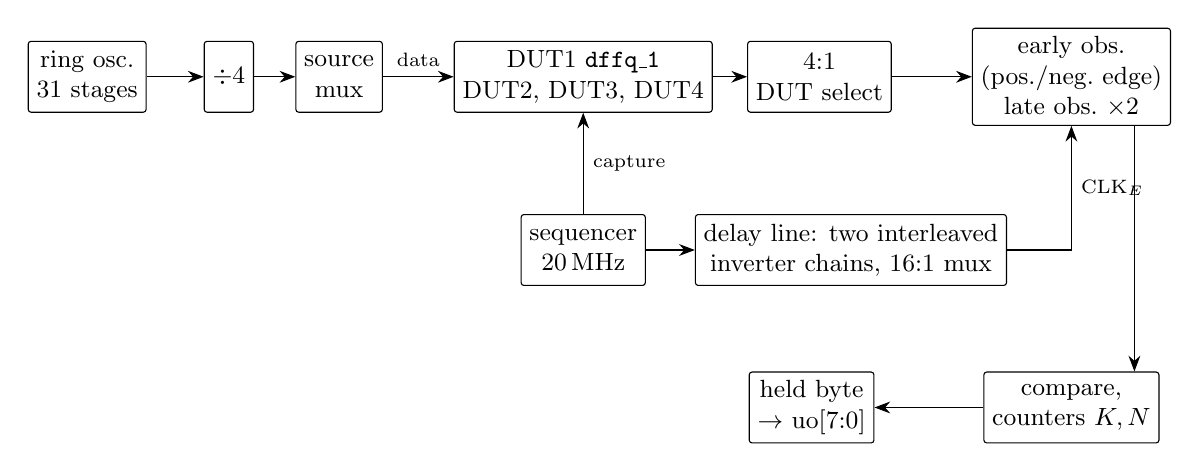
\begin{tikzpicture}[font=\small,
  box/.style={draw, rounded corners=1pt, minimum height=9mm, align=center, inner sep=3pt},
  arr/.style={-{Stealth[length=2mm]}}]
\node[box] (ring) at (0,0) {ring osc.\\31 stages};
\node[box] (div) at (1.8,0) {$\div4$};
\node[box] (src) at (3.2,0) {source\\mux};
\node[box] (duts) at (6.3,0) {DUT1 \texttt{dffq\_1}\\DUT2, DUT3, DUT4};
\node[box] (sel) at (9.3,0) {4:1\\DUT select};
\node[box] (obs) at (12.5,0) {early obs.\\(pos./neg.\ edge)\\late obs.\ $\times2$};
\node[box] (seq) at (6.3,-2.2) {sequencer\\20\,MHz};
\node[box] (dl) at (9.7,-2.2) {delay line: two interleaved\\inverter chains, 16:1 mux};
\node[box] (cnt) at (12.5,-4.2) {compare,\\counters $K,N$};
\node[box] (rd) at (9.2,-4.2) {held byte\\$\to$ uo[7:0]};
\draw[arr] (ring) -- (div); \draw[arr] (div) -- (src); \draw[arr] (src) -- node[above]{\scriptsize data} (duts);
\draw[arr] (duts) -- (sel); \draw[arr] (sel) -- (obs);
\draw[arr] (seq) -- node[right]{\scriptsize capture} (duts);
\draw[arr] (seq) -- (dl);
\draw[arr] (dl.east) -| node[pos=0.75,right]{\scriptsize CLK$_E$} (obs.south);
\draw[arr] ($(obs.south)+(0.8,0)$) -- ($(cnt.north)+(0.8,0)$);
\draw[arr] (cnt) -- (rd);
\end{tikzpicture}
\caption{Instrument block diagram. Only held counts leave the chip; picosecond timing never does.}
\end{figure}

\subsection{Delay line (sized from measured GF180 delays)}
Measured single-stage delays at TT 3.3\,V, each stage loaded by one mux input: inverter 90.4\,ps (70.2--123.9 across
conditions), inverter pair 160.2, \texttt{buf\_1} 182.0, \texttt{clkbuf\_1} 168.8, \texttt{dlya\_1} 346.2; 8:1 mux path
647.3\,ps; DUT-select \texttt{mux4\_1} 322.5\,ps; \texttt{xor2\_1} 359.3\,ps; ring period 4.51\,ns (3.46--6.25\,ns).
\begin{itemize}
\item \textbf{Why the design is what it is.} Each DUT is countable only inside a window of early delays: after its
  clock-to-Q plus the DUT-select mux delay, the observer's setup time and a 100\,ps margin, and before the
  disagreement probability falls below $10^{-6}$ (400 counts in about 27\,min at 243{,}000 effective trials/s). At TT 3.3\,V the windows (in code delay) are dffq\_1 1.03--1.71\,ns, DUT2 0.88--1.28, DUT3
  0.88--1.32, DUT4 0.88--1.67. DUT2's window is only about 4.4 single-inverter steps wide.
\item \textbf{Frozen design.} Two chains of eight \texttt{inv\_1} stages, the second offset by one extra inverter
  (about half a step), give 16 codes about 45\,ps apart. A 16:1 mux from five \texttt{mux4\_1} cells has about the
  delay of the old 8:1 path. Odd taps are inverted; a negative-edge early observer (\texttt{dffnq\_1}) samples them,
  with a \texttt{mux2\_1} choosing the observer output (no delay added to the clock path). On-chip calibration
  measures every code's actual delay.
\item \textbf{Predicted coverage.} At least 8 usable codes for every DUT at every condition (9 in most cases), for
  any chain offset between 0.25 and 0.75 of a step and a 16:1 mux delay between 0.9 and 1.25 times the old 8:1 path,
  with the base delay set at layout to 0 or 1 inverter (target: 5). The model assumes one side of the balance point is
  visible per DUT, as found in simulation.
\item \textbf{Stimulus.} Ring oscillator divided by 4 (was 64): a periodic data edge every 9\,ns at TT
  (6.9--12.5\,ns across conditions), at random phase to the capture clock. This raises every event rate and saves
  four divider flip-flops. The edge spacing is more than 20 times the largest DUT setup time at every condition,
  so a previous edge never falls inside a capture's setup window.
\end{itemize}

\subsection{Pins}
\begin{table}[H]
\centering\small
\begin{tabular}{@{}lll@{}}
\toprule
Pin & Direction & Function \\
\midrule
clk, rst\_n, ena & in & 20\,MHz system clock, reset, enable \\
ui[2:0] & in & delay code bits 0--2 \\
ui[3] & in & DUT select bit 0 \\
ui[4] & in & START \\
ui[5] & in & source select (ring or external) \\
ui[6] & in & external data \\
ui[7] & in & mode (measure or calibrate) \\
uio[0] & in & ring enable \\
uio[6] & in & \textbf{DUT select bit 1 (new)} \\
uio[7] & in & \textbf{delay code bit 3 (new)} \\
uo[7:0] & out & held count byte ($K$ or $H$) \\
uio[1], uio[2], uio[3] & out & BUSY, DONE, FAULT \\
uio[4], uio[5] & out & source monitor, trial monitor \\
\bottomrule
\end{tabular}
\caption{Pin assignment. No spare pins remain.}
\end{table}

\subsection{Transistor budget}
\begin{table}[H]
\centering\small
\begin{tabularx}{\linewidth}{@{}Xr@{}}
\toprule
Change against the 25 Sep design (1{,}790 planned + 210 reserve) & MOS \\
\midrule
DUT block: \texttt{dffq\_1} + three NAND flip-flops (150) replacing \texttt{dffq\_1} + \texttt{dffrnq\_1} (52) & $+98$ \\
4:1 DUT selector (\texttt{mux4\_1}) replacing 2:1 (\texttt{mux2\_1}) & $+14$ \\
Delay line (2 chains, 16:1 mux, negative-edge observer) and $\div4$ divider, against 8 taps, 8:1 mux, $\div64$ & $\approx 0$ to $+2$ \\
\midrule
Total change / reserve remaining & $\approx+114$ / $\approx96$ \\
\bottomrule
\end{tabularx}
\caption{Budget. The old delay line is modelled as eight \texttt{buf\_1} taps and an 8:1 mux, and the
\texttt{dffnq\_1} count is assumed equal to \texttt{dffq\_1}'s. Recount from the netlist at RTL freeze.}
\end{table}

%=====================================================================
\section{Novelty and prior art}
\begin{table}[H]
\centering\small
\begin{tabularx}{\linewidth}{@{}p{0.34\linewidth}X@{}}
\toprule
Prior work & What it establishes / what we add \\
\midrule
$\tau\approx C/g_m$; symmetric-latch analysis; optimal $W_n=W_p$ (square law) \cite{portmann1995} & Established physics. We add the allocation criterion for \emph{unequal} stages and its counter-intuitive half. \\
Unbalanced latch loads \cite{jeppson1996} & Small- and large-signal analysis of mismatch. The allocation rule for $\tau$ may be implicit there; full text to be checked. \\
Synchronizer guidelines \cite{beer2015} & External knobs with the cell fixed. We change the inside of the flip-flop, with standard cells. \\
Feedback flip-flops slower than library \cite{beer2011} & The observation. We give a criterion that predicts when added drive helps or hurts, and test both placements. \\
Gain boost during metastability \cite{zhou2006}; synchronizer with decreased resolving time (US~6{,}895{,}061); lightly loaded synchronizer latch (Oracle, US~8{,}552{,}779 \cite{oracle2013}) & The Oracle patent states that sizing chosen for data-path flip-flops can hurt synchronizer robustness, and uses lightly loaded cross-coupled transistors. New here: a quantitative criterion for where added drive helps, the demonstration that forward-side strengthening \emph{raises} $\tau$, a standard-cell realization, and a silicon test in GF180. \\
SKY130 metastability characterizer (Tiny Tapeout) & Different process and purpose (measurement only). Related work. \\
\bottomrule
\end{tabularx}
\caption{Positioning. ``New'' is to the best of our current search.}
\end{table}
\begin{checkbox}{Novelty checks still to do}
Read Jeppson \cite{jeppson1996} in full; read the claims of US~8{,}552{,}779 and US~6{,}895{,}061 in full (numbers
and titles verified); search NAND/SR-latch synchronizer literature for published $\tau$ comparisons against library
flip-flops; search GF180 metastability measurements.
\end{checkbox}

%=====================================================================
\section{Risks and open items}
\begin{table}[H]
\centering\small
\begin{tabularx}{\linewidth}{@{}p{0.32\linewidth}X@{}}
\toprule
Risk / item & Status and mitigation \\
\midrule
Silicon differs from SPICE & The experiment. Predicted differences 5--29\% against a $\pm3\%$ ratio-precision target. \\
Ratio precision $\pm3\%$ & To be shown in the error budget: with about 400 counts per code and 5 or more codes, statistical precision is about 1--2\% per $\tau$. \\
One-sided visibility and DUT4 curvature & Every DUT shows only one side of its balance point on chip (its slave leans one way); the event-rate model includes this. DUT4's fit curves slightly (knee fit 3--35\% above linear); a larger $\tau_4$ only widens the contrast. \\
SS-corner verdict & Disclosed (Section~\ref{sec:evidence}); direction holds. \\
Chip-to-chip and within-die mismatch & Measure every available die; compare ratios on the same die. \\
Flow modifies hand-placed cells & All DUT and delay-line instances and their nets must be \texttt{dont\_touch}. \\
Unmeasured: 16:1 mux path, offset inverter & Coverage shown robust over the plausible range; calibration measures actual delays. \\
NAND flip-flop setup time (4.2--5.0$\times$) & Not in the MTBF formula; state as a trade-off. \\
Supply voltage & Simulated at 3.0--3.6\,V per the design document; the library is rated for 5\,V. Confirm the shuttle's core supply; a 5\,V rerun takes about 75\,min. \\
RTL simulation & NAND DUT outputs are X until two clock edges; tests must not check them earlier. \\
Beer et al.\ variant numbers & Confirm against the paper (box in Section~\ref{sec:beer}). \\
\bottomrule
\end{tabularx}
\end{table}

%=====================================================================
\section{Plan}
\begin{itemize}
\item \textbf{1 Oct:} proposal talk (5 min). \textbf{8 Oct:} design review. \textbf{5 Nov:} timing review.
  \textbf{26 Nov:} system-verification milestone. \textbf{7 Dec 2026:} GF shuttle closes.
  Silicon expected around June 2027.
\item \textbf{Owners:} Ben --- circuits, physics, SPICE, delay line; Roshan --- sequencer, counters, readout, cocotb verification.
\item \textbf{Next steps:} integrate \texttt{meta\_duts.v}; implement the interleaved delay line, negative-edge observer,
  $\div4$ divider and new pins; recount transistors; write the error budget; update the design document and slides;
  optionally measure the 16:1 mux path and offset inverter (about 15\,min).
\end{itemize}

%=====================================================================
\section{Reproducibility and handoff}
\begin{itemize}
\item \textbf{Scripts:} \texttt{tau\_gf180.py} (DUT simulation, $\tau$ extraction, criteria, Verilog generation),
  SHA-256 \texttt{8c19ec6b\ldots e4f99fa}; \texttt{instr\_gf180.py} (instrument characterization and delay-line
  sizing), SHA-256 \texttt{e54aaacd\ldots 1513301}; \texttt{README.md}. Each has a \texttt{--selftest} mode that runs without ngspice.
\item \textbf{Environment:} ngspice-42; GF180 PDK \texttt{gf180mcuD} at ciel hash \texttt{1689ac3f\ldots}, built with
  open\_pdks' installer from \texttt{gf180mcu\_fd\_pr} \texttt{4d0b4cef\ldots} and \texttt{gf180mcu\_fd\_sc\_mcu7t5v0}
  \texttt{0ef8889a\ldots}; \texttt{.spiceinit}: \texttt{set ngbehavior=hs}. In the cloud sandbox use
  \texttt{--workers 2} (four parallel ngspice processes ran about $20\times$ slower each).
\item \textbf{Commands:} \texttt{python3 tau\_gf180.py --selftest}; \texttt{--smoke}; full run
  (about 75\,min at two workers); \texttt{python3 instr\_gf180.py} (about 10\,min).
\end{itemize}
\begin{table}[H]
\centering\small
\begin{tabularx}{\linewidth}{@{}lX@{}}
\toprule
Run & Outcome and fix \\
\midrule
1 & Saddle locator required three equilibria; the stable ones lie at the rails. Fixed: unique rising zero. \\
2 & \texttt{chgtol=1e-18} aborted every transient. Fixed; truncated waveforms now rejected; bisection made primary after a 12\% saddle gap. \\
3 & \texttt{abstol=1e-15} aborted loop-pin A1 decks. Fixed; one logged retry with looser tolerances added. \\
4 & DUT4 had no $\tau$: its slave pre-decides. Fixed: two-sided resample. \\
5 & \textbf{Final DUT results} (this document). \\
6 & Instrument: GF180 cells about $2\times$ slower than assumed; best design 2 codes. \\
7 & Single-inverter taps: best 4 codes; XOR too slow. Interleaved chains give at least 8 (analysis on measured delays). \\
\bottomrule
\end{tabularx}
\caption{Run history. All runs used the scripts unmodified by the executor; every fix was made by us and hashed.}
\end{table}

%=====================================================================
\section{Path to a paper}
\begin{itemize}
\item \textbf{Headline:} where added drive goes decides whether a flip-flop resolves metastability faster or slower;
  keeper-side allocation lowers $\tau$, forward-side allocation raises it, and a NAND-cell flip-flop with the
  favourable allocation has 36--47\% lower $\tau$ than the library cell.
\item \textbf{Figures:} the law (Figure~\ref{fig:law}), $\tau$ across conditions (Figure~\ref{fig:cond}), silicon
  $\ln\hat p$ against $d_k$ for all four DUTs, SPICE against silicon, MTBF impact (Figure~\ref{fig:tres}).
\item \textbf{Integrity:} criteria and SPICE predictions timestamped before silicon; raw counts, calibration records
  and die IDs kept from day one; release RTL, SPICE decks and counts with the paper.
\end{itemize}

%=====================================================================
\begin{thebibliography}{9}\small
\bibitem{beer2011} S.~Beer, R.~Ginosar, M.~Priel, R.~Dobkin, A.~Kolodny, ``An on-chip metastability measurement
circuit to characterize synchronization behavior in 65nm,'' \emph{Proc.\ IEEE ISCAS}, pp.~2593--2596, 2011,
doi:10.1109/ISCAS.2011.5938135.
\bibitem{beer2010} S.~Beer, R.~Ginosar, M.~Priel, R.~Dobkin, A.~Kolodny, ``The devolution of synchronizers,''
\emph{Proc.\ IEEE ASYNC}, 2010.
\bibitem{beer2015} S.~Beer, R.~Ginosar, ``Eleven ways to boost your synchronizer,'' \emph{IEEE Trans.\ VLSI Systems},
23(6):1040--1049, 2015.
\bibitem{portmann1995} C.~L.~Portmann, ``Characterization and reduction of metastability errors in CMOS interface
circuits,'' Ph.D.\ thesis, Stanford University, CSL-TR-95-671, 1995.
\bibitem{jeppson1996} K.~O.~Jeppson, ``Comments on the metastable behavior of mismatched CMOS latches,''
\emph{IEEE J.\ Solid-State Circuits}, 1996.
\bibitem{zhou2006} J.~Zhou, D.~Kinniment, G.~Russell, A.~Yakovlev, ``A robust synchronizer,'' \emph{Proc.\ IEEE ISVLSI}, 2006.
\bibitem{oracle2013} I.~W.~Jones, S.~Yang, M.~R.~Greenstreet, H.~N.~Gaywala, R.~J.~Drost, ``Synchronizer latch circuit
that facilitates resolving metastability,'' US Patent 8{,}552{,}779 B2 (Oracle), 2013.
\bibitem{ginosar2011} R.~Ginosar, ``Metastability and synchronizers: a tutorial,'' \emph{IEEE Design \& Test of
Computers}, 28(5), 2011.
\end{thebibliography}

\appendix
%=====================================================================
\section{Verilog of the devices under test (final)}
\label{app:verilog}
Generated by \texttt{tau\_gf180.py} in run 5 (loop feedback on A1; DUT3 keeper $\times2$). DUT3 and DUT4 differ from
DUT2 only in the cell size of \texttt{u\_mkp} and \texttt{u\_mfw} respectively.
\begin{lstlisting}
module meta_dut2 (input wire d, input wire clk, output wire q);
    wire clkn, g1, g2, mq, mqb, s1, s2, sqb;
    (* keep *) gf180mcu_fd_sc_mcu7t5v0__inv_1   u_cki (.I(clk), .ZN(clkn));
    (* keep *) gf180mcu_fd_sc_mcu7t5v0__nand2_1 u_mg1 (.A1(d),   .A2(clkn), .ZN(g1));
    (* keep *) gf180mcu_fd_sc_mcu7t5v0__nand2_1 u_mg2 (.A1(g1),  .A2(clkn), .ZN(g2));
    (* keep *) gf180mcu_fd_sc_mcu7t5v0__nand2_2 u_mfw (.A1(mqb), .A2(g1),   .ZN(mq));   // forward
    (* keep *) gf180mcu_fd_sc_mcu7t5v0__nand2_1 u_mkp (.A1(mq),  .A2(g2),   .ZN(mqb));  // keeper
    (* keep *) gf180mcu_fd_sc_mcu7t5v0__nand2_1 u_sg1 (.A1(mq),  .A2(clk),  .ZN(s1));
    (* keep *) gf180mcu_fd_sc_mcu7t5v0__nand2_1 u_sg2 (.A1(s1),  .A2(clk),  .ZN(s2));
    (* keep *) gf180mcu_fd_sc_mcu7t5v0__nand2_1 u_sfw (.A1(sqb), .A2(s1),   .ZN(q));
    (* keep *) gf180mcu_fd_sc_mcu7t5v0__nand2_1 u_skp (.A1(q),   .A2(s2),   .ZN(sqb));
endmodule
// meta_dut3: identical except u_mkp is nand2_2 (keeper x2)
// meta_dut4: identical except u_mfw is nand2_4 (forward x4)

module meta_duts (input wire d, input wire cap, output wire [3:0] q);
    (* keep *) gf180mcu_fd_sc_mcu7t5v0__dffq_1 u_dut1 (.CLK(cap), .D(d), .Q(q[0]));
    meta_dut2 u_dut2 (.d(d), .clk(cap), .q(q[1]));
    meta_dut3 u_dut3 (.d(d), .clk(cap), .q(q[2]));
    meta_dut4 u_dut4 (.d(d), .clk(cap), .q(q[3]));
endmodule
\end{lstlisting}

%=====================================================================
\section{Full SPICE results}
\begin{table}[H]
\centering\footnotesize
\begin{tabular}{@{}llrrrrr@{}}
\toprule
Condition & DUT & $\tau$ (ps) & $R^2$ & points & side & saddle (ps, diag.) \\
\midrule
\multirow{4}{*}{TT 3.3\,V} & dffq\_1 & 102.7 & 0.99999 & 24 & new & --- \\
& DUT2 & 64.5 & 0.99985 & 24 & new & 66.3 \\
& DUT3 & 57.5 & 1.00000 & 24 & new & 59.0 \\
& DUT4 & 71.9 & 0.99882 & 23 & old & 77.2 \\
\midrule
\multirow{4}{*}{SS 3.3\,V} & dffq\_1 & 133.7 & 1.00000 & 24 & new & --- \\
& DUT2 & 89.7 & 0.99992 & 24 & new & 90.3 \\
& DUT3 & 85.4 & 0.99263 & 23 & new & 80.4 \\
& DUT4 & 102.0 & 1.00000 & 23 & old & 104.7 \\
\midrule
\multirow{4}{*}{FF 3.3\,V} & dffq\_1 & 84.6 & 0.99992 & 24 & new & --- \\
& DUT2 & 51.6 & 0.99997 & 24 & new & 52.2 \\
& DUT3 & 45.2 & 0.99999 & 24 & new & 46.5 \\
& DUT4 & 57.6 & 0.99941 & 11 & old & 61.0 \\
\midrule
\multirow{4}{*}{TT 3.0\,V} & dffq\_1 & 111.7 & 1.00000 & 24 & new & --- \\
& DUT2 & 72.3 & 0.99995 & 24 & new & 73.3 \\
& DUT3 & 63.7 & 1.00000 & 24 & new & 65.3 \\
& DUT4 & 82.4 & 0.99998 & 23 & old & 85.3 \\
\midrule
\multirow{4}{*}{TT 3.6\,V} & dffq\_1 & 94.1 & 0.99677 & 24 & new & --- \\
& DUT2 & 60.4 & 0.99998 & 24 & new & 61.0 \\
& DUT3 & 52.8 & 0.99994 & 24 & new & 54.3 \\
& DUT4 & 68.0 & 0.99989 & 24 & old & 71.1 \\
\bottomrule
\end{tabular}
\caption{All bisection fits (run 5). ``Side'' is the side of the balance point whose output transition carries the
resolution.}
\end{table}

%=====================================================================
\section{Glossary}
\begin{description}[leftmargin=0pt,style=nextline]
\item[$\tau$] Metastability resolution time constant: the latch's unstable-mode time constant; the time for its
imbalance to grow by a factor $e$.
\item[MTBF] Mean time between failures: the average time between moments when a synchronizer is still undecided when it is read.
\item[synchronizer] A flip-flop that receives a signal from an unrelated clock domain.
\item[settling time $S$] The time a design allows a synchronizer to decide before its output is used.
\item[$T_W$, $f_C$, $f_D$] Metastability window (how wide a range of data timing causes trouble), clock frequency, data transition rate.
\item[transconductance $g$ / capacitance $C$] A gate's drive (output current per volt of input) / a node's load (charge per volt).
\item[TT, SS, FF] Typical, slow and fast transistor model corners.
\item[pre-registration] Fixing the test and its pass/fail criteria in writing before seeing the results.
\item[forward / keeper] The two loop NANDs of the master latch. The forward NAND drives \texttt{mq}, which feeds the slave; the keeper NAND drives \texttt{mqb}.
\item[$\delta$, $\delta^*$, $u$] Data-to-clock offset; the offset at which the flip-flop balances; $u=|\delta-\delta^*|$.
\item[early/late method] Sample the output after a short delay and again much later; a disagreement means unresolved at the short delay \cite{beer2011}.
\item[code window] The early delays at which a DUT is both past normal propagation and still countable ($p\ge10^{-6}$).
\end{description}

\end{document}
